\documentclass{article}
\usepackage[margin=1in]{geometry}
\usepackage{amsmath}
\usepackage{amssymb}
\usepackage{graphicx}
\usepackage{svg}
\usepackage{comment}
\usepackage{float}
\usepackage{cancel}
\usepackage{enumerate}
\usepackage[italicdiff]{physics}
\usepackage{dsfont}
\usepackage{hyperref}
\usepackage{siunitx}
% Display code
\usepackage{minted}
\usepackage{listings}
% Display graphs/figures
\usepackage{tikz}
\usepackage{hhline}
\hypersetup{
    colorlinks=true,
    linkcolor=blue,
    filecolor=blue,
    urlcolor=blue,
}
% Display boxes
\usepackage{tcolorbox}
\definecolor{lblue}{rgb}{0, 0.69, 1}

% Static title
\newtcolorbox{quickcheck}{fonttitle=\bfseries, title=Quick check}
\newtcolorbox{note}{colback=blue!5!white, colframe=blue!75!black,
fonttitle=\bfseries, title=Note}
\newtcolorbox{keyideas}{colback=green!5!white, colframe=green!75!black,
fonttitle=\bfseries, title=Key ideas}
\newtcolorbox{summary}{colback=green!5!white, colframe=green!75!black,
fonttitle=\bfseries, title=Summary}
\newtcolorbox{admin}{colback=yellow!5!white, colframe=yellow!90!black,
fonttitle=\bfseries, title=Administrivia}
% Editable title
\newtcolorbox{theorem}[1]{colback=lblue!5!white, colframe=lblue!75!black,
fonttitle=\bfseries, title=#1}
\newtcolorbox{problem}[1]{colback=red!5!white, colframe=red!75!black,
fonttitle=\bfseries, title=#1}
\newtcolorbox{example}[1]{colback=white, colframe=black,
fonttitle=\bfseries, title=#1}
\newtcolorbox{exercise}[1]{colback=orange!5!white, colframe=orange!95!black,
fonttitle=\bfseries, title=#1}
\newtcolorbox{strategy}[1]{colback=yellow!5!white, colframe=yellow!50!white, coltitle=black,
fonttitle=\bfseries, title=#1}
\newtcolorbox{definition}[1]{colback=green!5!white, colframe=green!75!black,
fonttitle=\bfseries, title=#1}

\newcommand{\sign}{\mathrm{sign}}

\newcommand{\RR}{\mathbb{R}}
\newcommand{\CC}{\mathbb{C}}

\newcommand{\cF}{\mathcal{F}}

% Start doc

\begin{document}
\title{Phyll-ed Notes, Lecture 4: Graphs, DFS, SCCs}
\author{CS124 - Spring 2023}
\date{Andrew Holmes --- 10 January 2023 --- version 1.0}
\maketitle

\tableofcontents

% \section{Admininstriva/Key ideas}
% \begin{admin}
%     \begin{itemize}
%         \item PSET 1 due today
%         \item PSET 2 out later today (due in 2 weeks)
%     \end{itemize}
% \end{admin}

% \begin{keyideas}
%     \begin{itemize}
%         \item What is a graph? Why might graphs be useful? How can we represent graphs?
%         \item Depth-First Search (DFS)
%         \begin{itemize}
%             \item Correctness, time \& space complexity
%             \item Properties \& types of edges
%             \item Topological sort
%         \end{itemize}
%         \item Strongly connected components (SCCs)
%     \end{itemize}
% \end{keyideas}

\newpage
\section{Graphs}
\subsection{Graph introduction}
A graph is a data structure consisting of a set of vertices and a set of edges between vertices. 
\begin{figure}[h]
    \centering
    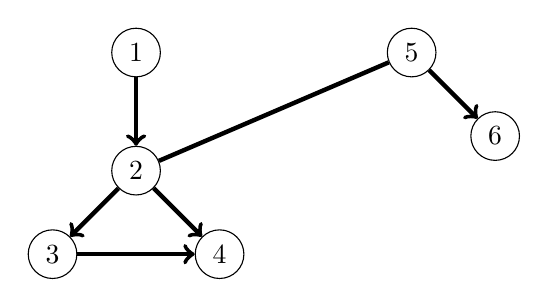
\begin{tikzpicture}[main/.style = {draw, circle}, node distance={15mm}] 
        \node[main] (1) {$1$}; 
        \node[main] (2) [below of=1] {$2$};
        \node[main] (3) [below left of=2] {$3$};
        \node[main] (4) [below right of=2] {$4$};
        \node[main] (5) [xshift=3.5cm] {$5$};
        \node[main] (6) [below right of=5] {$6$};
        \draw[->, ultra thick] (1) -- (2);
        \draw[->, ultra thick] (2) -- (3);
        \draw[->, ultra thick] (2) -- (4);
        \draw[->, ultra thick] (3) -- (4);
        \draw[->, ultra thick] (5) -- (6);
        \draw[-, ultra thick] (5) -- (2);
    \end{tikzpicture}
    \caption{A basic graph}
    \label{graph-intro-graph}
\end{figure}

While this visual description of a graph is most intuitive to humans, computers may not appreciate my struggle with \textit{tikz} to make pretty graphs, and thus we will generally define graphs in mathematical notation as:
\begin{equation}
    G = (V(G), E(G))
\end{equation}
Thus our graph is simply a tuple of the vertices and edges that make up the graph. Breaking this down further:

\begin{itemize}
    \item $V(G)$ is a set/list of vertices in the graph. We generally number them $\{0, 1, ..., n-1\}$.
    \item $E(G)$ is a set/list of edges in the graph, such as (for example) $\{(0, 1), (3, 5)\}$.
\end{itemize}

The edges in $E(G)$ are \textbf{directed}, such that each tuple $(u, v)$ corresponds to an edge \textbf{from} $u$ \textbf{to} $v$. For an undirected edge (an edge where we can travel from $u$ to $v$ and from $v$ to $u$), both $(u,v)$ and $(v,u)$ must be in $E(G)$. A graph is \textit{undirected} if and only if $\forall (u, v) \in E(G), (v, u) \in E(G)$. Else the graph is \textit{directed}.

A graph's edges may also have \textbf{weights} (or lengths) associated with edges. In this case we consider the graph to have a corresponding function
\begin{equation}
    f: E(G) \mapsto \mathbb{R}
\end{equation}
This is simply a function that takes in an edge and outputs a real number, which is the weight associated with the input edge.

\begin{quickcheck}
    Let's consider the graph in \ref{graph-intro-graph}. Fill in $V(G)$ and $E(G)$ for this graph:
    \begin{align*}
        V(G) &= \{1, 2, 3, 4, 5, 6 \}\\
        E(G) &= \{(1, 2), (2, 3), (3, 4), (2, 4), (5, 6), (2, 5), (5, 2) \}
    \end{align*}
\end{quickcheck}

\begin{problem}{Problem 1: Modelling problems with graphs}
    What are some things we might model with graphs?
\end{problem}

Some natural real-world problems we might model with graphs include transportation problems. We could model cities as vertices and roads connecting them as edges, or airports as vertices and flight paths as edges. For both of these cases, we might also associate some extra information with each edge - for example, the expected time to complete the journey, or the cost. Another important set of problems is modelling networks (such as telecom networks). For each of these, we might be interested in finding the shortest distance between two points, the maximum traffic possible along a route or other information.

\subsection{Graph representation}
\begin{problem}{Problems 2 \& 3: Graph representation}
    How can we represent a graph? How should we represent a graph?
\end{problem}

There are two primary ways to represent a graph: the \textit{adjacency matrix} representation and the \textit{adjacency list} representation.

The \textbf{adjacency matrix} for a graph $G$ with $n$ vertices is a $n \times n$ matrix $A$, where $A_{i, j} = 1 \iff (i, j) \in E(G)$ and $A_{i, j} = 0$ otherwise. 

The advantage of the adjacency matrix representation is that it takes constant time (just one memory access) to determine whether or
not there is an edge between any two given vertices. The disadvantage of the adjacency matrix representation is that it requires $\Omega (n^2)$ storage, even if the graph has as few as $O(n)$ edges. Moreover, just examining all the entries of the matrix would require $\Omega (n^2)$ steps, thus precluding the possibility of linear time algorithms for graphs with $o(n^2)$ edges (at least in cases where all the matrix entries must be examined). In scenarios when edges have associated lengths/weights, the adjacency matrix can be modified to contain the length/weight instead of just a 1 (although there needs to be some care taken, imagine there was a 0 weight edge from $u$ to $v$ - this could appear as no edge if we use this idea carelessly).

The \textbf{adjacency list} for a graph $G$ with $n$ vertices is a length $n$ array, where the $i$th element points to the adjacency list of vertex $i$. The adjacency list of a vertex $i$ is a list that contains all vertices such that $(i, v) \in E(G)$ (in any order). 

The total storage used by an adjacency list representation of a graph with $n$ vertices and $m$ edges is $O(n+m)$, since the array has length $n$ (size $O(n)$), and the combined space of storing all of the elements within the adjacency lists must be $O(m)$, as for each edge we store one value. The adjacency list representation hence avoids the disadvantage of using more space than necessary. We will use this representation for all our graph algorithms that take linear or near linear time. A disadvantage of adjacency lists, however, is that determining whether there is an edge from vertex $i$ to vertex $j$ may take as many as $n$ steps, since there is no systematic shortcut to scanning the adjacency list of vertex i. For applications where determining if there is an edge between two vertices is the bottleneck, the adjacency matrix is thus preferable.

\begin{example}{Graph representation example}
    \begin{center}
    \begin{minipage}{.25\linewidth}

    \centering
    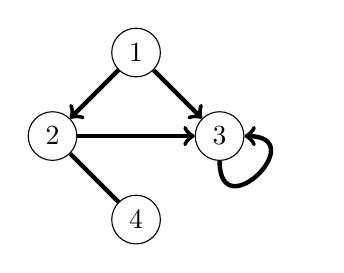
\begin{tikzpicture}[main/.style = {draw, circle}, node distance={15mm}] 
        \node[main] (1) {$1$};
        \node[main] (2) [below left of=1] {$2$};
        \node[main] (3) [below right of=1] {$3$};
        \node[main] (4) [below right of=2] {$4$};
        \draw[->, ultra thick] (1) -- (2);
        \draw[->, ultra thick] (2) -- (3);
        \draw[->, ultra thick] (1) -- (3);
        \draw[->, ultra thick] (3) to [out=270,in=0,looseness=5] (3);
        \draw[-, ultra thick] (2) to (4);
    \end{tikzpicture}
    \caption{Example graph}
    \label{graph-rep-ex}
\end{minipage}%
\begin{minipage}{.3\linewidth}
    \centering
    \begin{tabular}{|c||c|c|c|c|}
         \hline
         Vertex & 1 & 2 & 3 & 4 \\
         \hhline{|=||=|=|=|=|}
         1 & 0 & 1 & 1 & 0\\
         2 & 0 & 0 & 1 & 1\\
         3 & 0 & 0 & 1 & 0\\
         4 & 0 & 1 & 0 & 0\\
         \hline
    \end{tabular}
    \vspace{2mm}
    
    \caption{Adjacency matrix corresponding to graph}
    \label{tab:my_label}
\end{minipage}
\begin{minipage}{.25\linewidth}
    \centering
    \includegraphics[scale=0.35]{adj-list-ex.PNG}
    
    \caption{Adjacency list corresponding to graph}
    \label{tab:my_label}
\end{minipage}
\end{center}
\end{example}


\begin{note}
    We will often classify graphs into certain types:
    \begin{itemize}
        \setlength\itemsep{0.05em} 
        \item \textbf{Directed or undirected} (see 1.1: Graph introduction)
        \item \textbf{Cyclic or acyclic} - does the graph contain one or more cycles?
        \item \textbf{Connected} - exists a \textbf{path} between every pair of vertices (not necessarily a direct edge)
        \item \textbf{Complete} - exists an \textbf{edge} between every pair of vertices
        \item \textbf{Tree} - an undirected graph where any two vertices are connected by \textbf{exactly} one path
        \item \textbf{DAG} - a Directed Acyclic Graph.
    \end{itemize}
\end{note}

\newpage
\section{Depth-First Search (DFS)}

\subsection{DFS introduction}

There are two fundamental algorithms for searching a graph: \textbf{depth-first search} and \textbf{breadth-first search}. We will explore depth-first search this lecture, and breadth-first search next lecture.

Depth-First Search follows edges from vertex to vertex until it reaches a vertex it has already visited or a vertex with no outgoing edges, at which point it backtracks (reverses its steps) until it reaches a vertex that has outgoing edges that it has not explored yet. One famous example of DFS is exploring mazes:

\noindent
\begin{minipage}{.33\linewidth}
    \includegraphics[scale=0.37]{maze-DFS-1.PNG}
    
    % \caption{}
    \label{tab:my_label}
\end{minipage}
\begin{minipage}{.33\linewidth}
    \includegraphics[scale=0.37]{maze-DFS-2.PNG}
    
    % \caption{}
    \label{tab:my_label}
\end{minipage}
\begin{minipage}{.33\linewidth}
    \includegraphics[scale=0.37]{maze-DFS-3.PNG}
    
    % \caption{}
    \label{tab:my_label}
\end{minipage}

Looking at this example, DFS on this maze chooses to go right initially, and it explores this path as far as it can go, then backtracks back to the start square. Here there is another available path, so it explores down this path in the second image. At the next junction, it chooses to go right, and again explores this path until it can go no further before backtracking, and the same again in the third image. 

\begin{note}
    We can represent this maze as a graph, hence allowing us to run DFS! For example, the top left corner can be represented as the following graph:
    
    \centering
    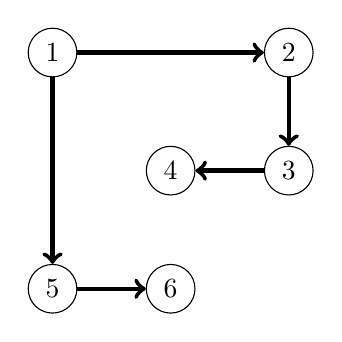
\begin{tikzpicture}[main/.style = {draw, circle}, node distance={15mm}] 
        \node[main] (1) {$1$};
        \node[main] (2) [right of=1, xshift=1.5cm] {$2$};
        \node[main] (3) [below of=2] {$3$};
        \node[main] (4) [left of=3] {$4$};
        \node[main] (5) [below of=1, yshift=-1.5cm] {$5$};
        \node[main] (6) [right of=5] {$6$};
        \draw[->, ultra thick] (1) -- (2);
        \draw[->, ultra thick] (2) -- (3);
        \draw[->, ultra thick] (3) -- (4);
        \draw[->, ultra thick] (1) to (5);
        \draw[->, ultra thick] (5) to (6);
    \end{tikzpicture}

    Our DFS started at vertex $1$, then went $1 \to 2 \to 3 \to 4$. $4$ is a leaf vertex/has no outgoing edges, so it backtracked to $1$. $1$ has another edge it can follow, so it searched that branch, following $1 \to 5 \to 6$ and so on.
\end{note}

\subsection{DFS and stacks}

Depth-First Search uses a \textbf{stack} to keep track of which vertices to explore next. A stack is a \textbf{last in, first out (LIFO)} data structure. This means that the last item we add to the stack is always the first to be removed. We generally refer to adding to a stack as \textbf{pushing/appending} to a stack, and removing an element as \textbf{popping} an element.

For example, in the dining hall the staff create a stack of trays. The last clean tray added is at the top, and when you arrive in the dining hall, the tray you collect is the top one (the last added). The person afer you collects a tray that was added to the stack before your one. If the stack was getting low, staff might come and add several more trays, such that the tray at the very bottom might have been added first, but never gets used. In this example, it would be possible, albeit a massive pain trying to remove the first clean tray from the bottom without removing the others. People here could break the normal stack order - when programming a stack, it's common to use an abstraction barrier to prevent actions like these. 

In DFS, when we find a vertex and explore its edges, we add each unvisited vertex accessible from one of these edges to the stack. We then pop (remove) one of them from the stack (the last one added), and repeat the process until our stack is empty. Let's explore an example in detail.

\begin{example}{DFS example}
    Let's break down how DFS ran on the maze graph:

    \centering

    \begin{minipage}{0.4\linewidth}
        \centering
        \textbf{Diagram}
    \end{minipage}
    \begin{minipage}{0.4\linewidth}
    \centering
        \textbf{Explanation}
    \end{minipage}
    \begin{minipage}{0.15\linewidth}
    \centering
        \textbf{Stack at end of step}
    \end{minipage} \\
    
    \begin{minipage}{0.4\linewidth}
    \centering
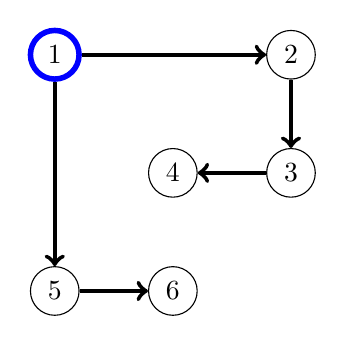
\begin{tikzpicture}[main/.style = {draw, circle}, node distance={15mm},   blacknode/.style={shape=circle, draw=black, line width=2},                              bluenode/.style={shape=circle, draw=blue, line width=2}]        \centering
        \node[bluenode] (1) {$1$};
        \node[main] (2) [right of=1, xshift=1.5cm] {$2$};
        \node[main] (3) [below of=2] {$3$};
        \node[main] (4) [left of=3] {$4$};
        \node[main] (5) [below of=1, yshift=-1.5cm] {$5$};
        \node[main] (6) [right of=5] {$6$};
        \draw[->, ultra thick] (1) -- (2);
        \draw[->, ultra thick] (2) -- (3);
        \draw[->, ultra thick] (3) -- (4);
        \draw[->, ultra thick] (1) to (5);
        \draw[->, ultra thick] (5) to (6);
    \end{tikzpicture}
    \end{minipage}
    \begin{minipage}{0.4\linewidth}
    \centering
        We start with the source vertex, and set it as visited. We push the two vertices we can reach from $1$ to the stack in some order, in this case $5$ and then $2$. 
    \end{minipage}
    \begin{minipage}{0.15\linewidth}
    \centering
        $\{5, 2\}$
    \end{minipage}   \\
    \begin{minipage}{0.4\linewidth}
    \centering
    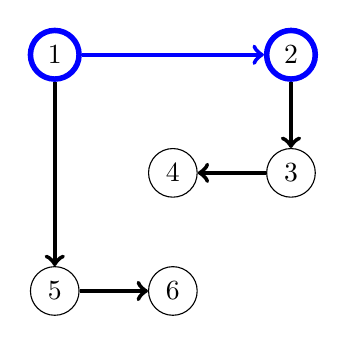
\begin{tikzpicture}[main/.style = {draw, circle}, node distance={15mm},                               bluenode/.style={shape=circle, draw=blue, line width=2}] 
    \centering
        \node[bluenode] (1) {$1$};
        \node[bluenode] (2) [right of=1, xshift=1.5cm] {$2$};
        \node[main] (3) [below of=2] {$3$};
        \node[main] (4) [left of=3] {$4$};
        \node[main] (5) [below of=1, yshift=-1.5cm] {$5$};
        \node[main] (6) [right of=5] {$6$};
        \draw[->, ultra thick, blue] (1) -- (2);
        \draw[->, ultra thick] (2) -- (3);
        \draw[->, ultra thick] (3) -- (4);
        \draw[->, ultra thick] (1) to (5);
        \draw[->, ultra thick] (5) to (6);
    \end{tikzpicture}
    \end{minipage}
    \begin{minipage}{0.4\linewidth}
    \centering
        We now pop $2$ from the stack and set it as visited. We push $3$ to the stack since it is the only unvisited vertex we can reach from $2$.
    \end{minipage}
    \begin{minipage}{0.15\linewidth}
    \centering
        $\{5, 3\}$
    \end{minipage}    \\
    \begin{minipage}{0.4\linewidth}
    \centering
    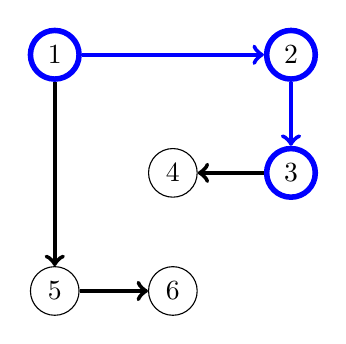
\begin{tikzpicture}[main/.style = {draw, circle}, node distance={15mm},                               bluenode/.style={shape=circle, draw=blue, line width=2}] 
    \centering
        \node[bluenode] (1) {$1$};
        \node[bluenode] (2) [right of=1, xshift=1.5cm] {$2$};
        \node[bluenode] (3) [below of=2] {$3$};
        \node[main] (4) [left of=3] {$4$};
        \node[main] (5) [below of=1, yshift=-1.5cm] {$5$};
        \node[main] (6) [right of=5] {$6$};
        \draw[->, ultra thick, blue] (1) -- (2);
        \draw[->, ultra thick, blue] (2) -- (3);
        \draw[->, ultra thick] (3) -- (4);
        \draw[->, ultra thick] (1) to (5);
        \draw[->, ultra thick] (5) to (6);
    \end{tikzpicture}
    \end{minipage}
        \begin{minipage}{0.4\linewidth}
    \centering
        We now pop $3$ from the stack and set it as visited.  We push $4$ to the stack since it is the only unvisited vertex we can reach from $3$.
    \end{minipage}
    \begin{minipage}{0.15\linewidth}
    \centering
        $\{5, 4\}$
    \end{minipage}\\
    \begin{minipage}{0.4\linewidth}
    \centering
    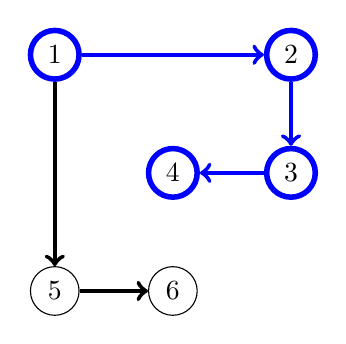
\begin{tikzpicture}[main/.style = {draw, circle}, node distance={15mm},                               bluenode/.style={shape=circle, draw=blue, line width=2}] 
    \centering
        \node[bluenode] (1) {$1$};
        \node[bluenode] (2) [right of=1, xshift=1.5cm] {$2$};
        \node[bluenode] (3) [below of=2] {$3$};
        \node[bluenode] (4) [left of=3] {$4$};
        \node[main] (5) [below of=1, yshift=-1.5cm] {$5$};
        \node[main] (6) [right of=5] {$6$};
        \draw[->, ultra thick, blue] (1) -- (2);
        \draw[->, ultra thick, blue] (2) -- (3);
        \draw[->, ultra thick, blue] (3) -- (4);
        \draw[->, ultra thick] (1) to (5);
        \draw[->, ultra thick] (5) to (6);
    \end{tikzpicture}
    \end{minipage}
    \begin{minipage}{0.4\linewidth}
    \centering
        We now pop $4$ from the stack and set it as visited.  There is nowhere to go from $4$, so we push nothing to the stack. Since only $5$ remains on the stack, we will explore $5$ next - this is where we encounter the idea of backtracking: we just explored $4$, but now we go back to one of the outgoing edges from $1$ since we have run out of paths on this branch.
    \end{minipage}
    \begin{minipage}{0.15\linewidth}
    \centering
        $\{5\}$
    \end{minipage}\\
    \begin{minipage}{0.4\linewidth}
    \centering
    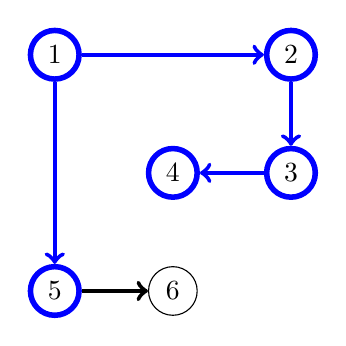
\begin{tikzpicture}[main/.style = {draw, circle}, node distance={15mm},                               bluenode/.style={shape=circle, draw=blue, line width=2}] 
    \centering
        \node[bluenode] (1) {$1$};
        \node[bluenode] (2) [right of=1, xshift=1.5cm] {$2$};
        \node[bluenode] (3) [below of=2] {$3$};
        \node[bluenode] (4) [left of=3] {$4$};
        \node[bluenode] (5) [below of=1, yshift=-1.5cm] {$5$};
        \node[main] (6) [right of=5] {$6$};
        \draw[->, ultra thick, blue] (1) -- (2);
        \draw[->, ultra thick, blue] (2) -- (3);
        \draw[->, ultra thick, blue] (3) -- (4);
        \draw[->, ultra thick, blue] (1) to (5);
        \draw[->, ultra thick] (5) to (6);
    \end{tikzpicture}    
    \end{minipage}
    \begin{minipage}{0.4\linewidth}
    \centering
        We now pop $5$ from the stack and set it as visited.  We push $6$ to the stack since it is the only unvisited vertex we can reach from $5$.
    \end{minipage}
    \begin{minipage}{0.15\linewidth}
    \centering
        $\{6\}$
    \end{minipage}\\
\end{example}

\newpage

\subsection{DFS pseudocode}

\begin{strategy}{DFS pseudocode (attempt 1)}
    Here's an attempt at writing some pseudocode for DFS:
    \begin{lstlisting}
    def search(v):
	explored(v) = 1
	previsit(v)
	for (v,w) in E:
		if explored(w) == 0:
			search(w)
	postvisit(v)
\end{lstlisting}
\end{strategy}
\begin{problem}{Problem 4: DFS pseudocode}
    Is this guaranteed to reach every node in a graph? When will it search all of $G$?
\end{problem}
Here are a number of scenarios when this won't search the whole graph:
\begin{itemize}
    \item The graph has multiple 'islands' where there are no edges between 'islands'. For example, consider the following graph:
    \begin{figure}[h]
        \centering
        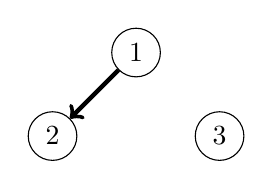
\begin{tikzpicture}[main/.style = {draw, circle}, node distance={15mm}] 
        \node[main] (1) {$1$};
        \node[main] (2) [below left of=1] {$2$};
        \node[main] (3) [below right of=1] {$3$};
        \draw[->, ultra thick] (1) -- (2);
    \end{tikzpicture}
        \caption{Problematic graph 1}
        \label{fig:my_label}
    \end{figure}
    
    No matter which vertex we start our search on, our current algorithm won't search the whole graph - there is no edge between vertex $3$ and vertices $1, 2$.
    \item We start searching at a vertex that cannot reach all vertices (although there may be only 1 'island):
        \begin{figure}[h]
        \centering
        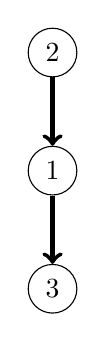
\begin{tikzpicture}[main/.style = {draw, circle}, node distance={15mm}] 
        \node[main] (2) {$2$};
        \node[main] (1) [below of=2] {$1$};
        \node[main] (3) [below of=1] {$3$};
        \draw[->, ultra thick] (1) -- (3);
        \draw[->, ultra thick] (2) -- (1);
    \end{tikzpicture}
        \caption{Problematic graph 2}
        \label{fig:my_label}
    \end{figure}

    Here if we ran DFS starting with vertex $1$ we would never reach vertex $2$.
\end{itemize}

\begin{strategy}{DFS pseudocode fix}
    Let's fix our pseudocode for DFS. We will use the previous version as a helper function to the main DFS function to fix our problems:
    \begin{lstlisting}[mathescape=true]
def search(v):
    explored(v) = 1
    previsit(v)
    for (v,w) in E:
        if explored(w) == 0:
            search(w)
    postvisit(v)
    \end{lstlisting}  


    \begin{lstlisting}
def DFS(G):
    for v in V(G):
        explored(v) = 0
    for v in V(G):
        if explored(v) == 0:
            search(v)
    \end{lstlisting}
\end{strategy}

\begin{note}
    Looking at our pseudocode above, there is no clear implementation or usage of a stack. This is because, by using recursion, we are using the \textbf{calling stack} implicitly to handle our stack for us. \lstinline{search(v)} is on the calling stack before \lstinline{search(w)}, and this is where the stack is hidden in this implementation. Here's an iterative implementation with an explicit stack, although without previsit/postvisit as this is trickier to do iteratively.

    \begin{lstlisting}
def DFS(self,s):
    for v in V(G):
        explored(v) = 0
    stack = []
    stack.append(s)
    while (stack not empty):
        v = stack.pop()
        explored(v) = 1
        for (v, w) in E(G):
            if (explored(w) == 0:
                stack.append(w)
    \end{lstlisting}
    
\end{note}

\subsection{DFS time complexity}

\begin{problem}{Problem 5: DFS time complexity}
    How long does DFS take to run?
\end{problem}
Running our DFS algorithm, we initally spend $O(n)$ time initializing the visited/explored set to zero. We then explore each vertex once, and for each vertex we explore all outgoing edges once within our search helper function. Thus the running time must be $O(n + m)$ as we use each edge and vertex only once.

\subsection{Postvisit/previsit}
So far we haven't discussed much what the $previsit$ and $postvisit$ functions do, except that we assumed they ran in $O(1)$ time for our time complexity analysis. For DFS, they simply increment a shared counter. To modify DFS' behaviour, it can be useful to change the $previsit$ and $postvisit$ functions, as we will see later.

\begin{example}{Previsit/postvisit example}
    Let's run DFS on the following graph, assuming it picks $1$ as the initial vertex and it will break ties in ascending vertex order (lowest vertex will always be picked first).

    \vspace{2mm}
    \begin{minipage}{0.5\linewidth}
    \centering
    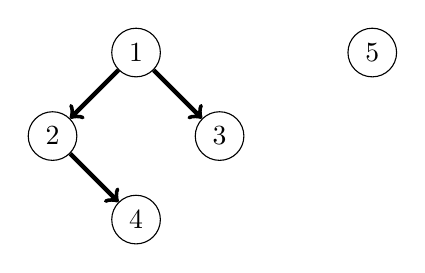
\begin{tikzpicture}[main/.style = {draw, circle}, node distance={15mm}] 
        \node[main] (1) {$1$};
        \node[main] (2) [below left of=1] {$2$};
        \node[main] (3) [below right of=1] {$3$};
        \node[main] (4) [below right of=2] {$4$};
        \node[main] (5) [xshift=3cm] {$5$};
        \draw[->, ultra thick] (1) -- (2);
        \draw[->, ultra thick] (1) -- (3);
        \draw[->, ultra thick] (2) -- (4);
    \end{tikzpicture}
    \end{minipage}
    \begin{minipage}{0.5\linewidth}
    \centering
    \begin{tabular}{|c|c|c|}
        \hline
        Vertex & Previsit & Postvisit  \\
        \hline
        1 & 1 & 8 \\
        2 & 2 & 5 \\
        3 & 6 & 7 \\
        4 & 3 & 4 \\
        5 & 9 & 10  \\
        \hline
    \end{tabular}
    \end{minipage}
\end{example}


\subsection{Types of edges}

When we run DFS on a graph, we can categorize the edges of the graph into 4 categories:

\begin{itemize}
    \item \textbf{Tree (actually forest) edges}: edges that reach a new vertex.
    \item \textbf{Forward edges}: edge from a vertex to non-child descendant.
    \item \textbf{Back edges}: edge from a vertex to ancestor.
    \item \textbf{Cross edges}: everything else.
\end{itemize}

\begin{figure}[h]
    \centering
        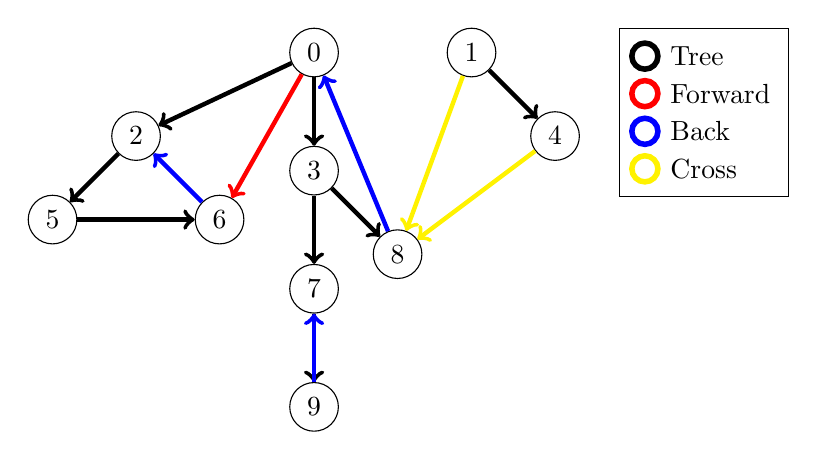
\begin{tikzpicture}[main/.style = {draw, circle}, node distance={15mm},   blacknode/.style={shape=circle, draw=black, line width=2},
  bluenode/.style={shape=circle, draw=blue, line width=2},
  yellownode/.style={shape=circle, draw=yellow, line width=2},
  rednode/.style={shape=circle, draw=red, line width=2}] 
        \node[main] (0) {$0$};
        \node[main] (1) [xshift=2cm] {$1$};
        \node[main] (2) [below left of=0, xshift=-1.2cm] {$2$};
        \node[main] (3) [below of=0] {$3$};
        \node[main] (4) [below right of=1] {$4$};
        \node[main] (5) [below left of=2] {$5$};
        \node[main] (6) [below right of=2] {$6$};
        \node[main] (7) [below of=3] {$7$};
        \node[main] (8) [below right of=3] {$8$};
        \node[main] (9) [below of=7] {$9$};
        \draw[->, ultra thick] (0) -- (2);
        \draw[->, ultra thick] (2) -- (5);
        \draw[->, ultra thick] (5) -- (6);
        \draw[->, ultra thick, blue] (6) -- (2);
        \draw[->, ultra thick] (0) -- (3);
        \draw[->, ultra thick, red] (0) -- (6);
        \draw[->, ultra thick] (3) -- (7);
        \draw[->, ultra thick] (7) -- (9);
        \draw[->, ultra thick] (3) -- (8);
        \draw[->, ultra thick, blue] (8) -- (0);
        \draw[->, ultra thick] (1) -- (4);
        \draw[->, ultra thick, yellow] (4) -- (8);
        \draw[->, ultra thick, yellow] (1) -- (8);
        \draw[->, ultra thick, blue] (9) -- (7);
        \matrix [draw,below right, xshift=0.5cm] at (current bounding box.north east) {
          \node [blacknode,label=right:Tree] {}; \\
          \node [rednode,label=right:Forward] {}; \\
          \node [bluenode,label=right:Back] {}; \\
          \node [yellownode,label=right:Cross] {}; \\
        };
    \end{tikzpicture}
    \caption{DFS edge type examples}
    \label{fig:my_label}
\end{figure}

\newpage

\subsection{DFS properties}
DFS has a number of useful properties that we will use in the future:

\begin{theorem}{DFS property 1}
    If $(u, v) \in E(G)$ then $(u, v)$ is a back edge $\iff postorder(u) < postorder(v)$.
\end{theorem}

\textbf{Proof}:

$(\Rightarrow)$ if $(u, v)$ is a back edge, then $v$ is an ancestor of $u$. In Depth-First Search, we explore all descendants of a node before backtracking, thus since $u$ is a descendant of $v$ we must explore and postvisit $u$ before $v$, hence $postorder(u) < postorder(v)$.

$(\Leftarrow)$ if $postorder(u) < postorder(v)$ and $(u, v) \in E(G)$ then $u$ must be a descendant of $v$. Let's assume for contradiction that $u$ is not a descendant of $v$. Then once we reached $u$, DFS would eventually explore the edge $(u, v)$ and reach $v$. Then it would explore all descendants of $v$ before backtracking to $u$ (or if $(u, v)$ were a cross edge, backtrack immediately), which would ensure $postorder(v) < postorder(u)$, a contradiction. Thus since $u$ is a descendant of $v$, $(u, v)$ by definition must be a back edge.

\begin{theorem}{DFS property 2}
    $G$ has a cycle $\iff$ DFS yields a back edge.    
\end{theorem}

\textbf{Proof}:

$(\Rightarrow)$ Let's assume for contradiction that $G$ has a cycle but DFS does not yield a back edge. Since there exists no back edges in the graph, there can not exist an edge from any vertex to an ancestor of that vertex. But we know there exists a cycle - for there to be a cycle, there must exist some path from a vertex $u$ that returns to $u$. Thus there must exist some descendant of $u$, $v$, such that there is an edge from $v$ to $u$. But since $u$ is an ancestor of $v$, by definition $(v, u)$ is a back edge and we have reached a contradiction. (\textit{Note: here we are not allowing edges from a vertex back to itself})

$(\Leftarrow)$ if DFS yields a back edge, then there exists some edge $(v, u) \in E(G)$ such that $u$ is an ancestor of $v$. Since $u$ is an ancestor of $v$, there exists some path from $u$ to $v$, and we know there is a path from $v$ to $u$ (namely the edge $(v, u)$, although there may be more), thus there exists a cycle in the graph.


\begin{problem}{Problem 6: DFS \& back edges}
    Is it possible that one DFS of a graph G yields a back edge, but another DFS yields no back edges?
\end{problem}

Using the second DFS property, if one DFS of $G$ yields a back edge, then $G$ has a cycle. Thus for any other DFS, we know that if $G$ has a cycle, DFS must yield a back edge, thus this is not possible.

\subsection{Topological sort}

\begin{problem}{Problen 7: Topological sort}
    Let's suppose you have a list of tasks where some tasks must be done before others. Is it always possible to order them?
\end{problem}

This is not always possible. Let's consider two tasks, buying your partner chocolate and finding out what chocolate they like without asking them (or, for this example, any of their friends etc). You need to know what chocolate they like to buy them chocolate, but you seem to have no other option but to buy them chocolate to find out what chocolate they like. Both tasks require the other task to be completed before being able to complete themselves - it's a cycle, and you are stuck (it's a cruel world)! Topological sorting is \textbf{not possible} on cyclic graphs.


\begin{problem}{Problem 8: Topogical sort 2}
    Topological Sort: you have a list of tasks; some tasks must be done before others. How to order them?
\end{problem}

Now assuming we have a DAG, is it possible to order/schedule them such that for any task, all prerequisite tasks are earlier in the oredering than the task (all prerequisite tasks are scheduled/completed before the task)? The answer is yes, using a topological ordering: 

\begin{definition}{Definition: Topological sort/ordering}
    A \textbf{topological sort} or \textbf{ordering} is a linear ordering of vertices such that for all edges $(u, v) \in E(G)$, $u$ comes before $v$ in the ordering.
\end{definition}

Finding a topological ordering is remarkably easy using our DFS knowledge:

\begin{strategy}{Topological sort algorithm}
    \begin{enumerate}
        \item Run DFS on the graph (which must be a DAG).
        \item Sort vertices by decreasing postorder number.
    \end{enumerate}   
\end{strategy}

\textbf{Proof that this gives a topological sort}: to prove this, we will use our two DFS properties. Firstly, by property 2, since we have a DAG, we know there are no back edges in the graph. Then from property two, we know for all edges $(u, v)$, $postorder(v) < postorder(u)$. Thus sorting by decreasing postorder number will give vertices in an order such that for any vertex $v$, any vertices with incoming edges to $v$ will be earlier in the ordering than $v$. In terms of task scheduling, this ensures that all tasks required by $v$ will be completed before $v$.

\begin{example}{Topological sort example} 
    \centering
    \begin{minipage}{0.4\linewidth}
    \centering
    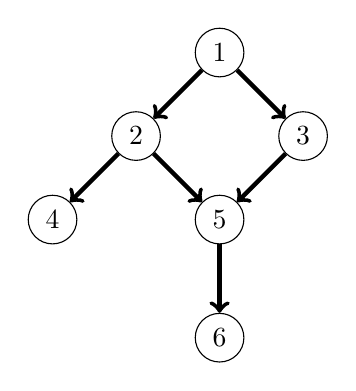
\begin{tikzpicture}[main/.style = {draw, circle}, node distance={15mm}] 
        \node[main] (1) {$1$};
        \node[main] (2) [below left of=1] {$2$};
        \node[main] (3) [below right of=1] {$3$};
        \node[main] (4) [below left of=2] {$4$};
        \node[main] (5) [below right of=2] {$5$};
        \node[main] (6) [below of=5] {$6$};
        \draw[->, ultra thick] (1) -- (2);
        \draw[->, ultra thick] (1) -- (3);
        \draw[->, ultra thick] (2) -- (4);
        \draw[->, ultra thick] (2) -- (5);
        \draw[->, ultra thick] (3) -- (5);
        \draw[->, ultra thick] (5) -- (6);
    \end{tikzpicture}
    \end{minipage}
    \begin{minipage}{0.4\linewidth}
    \centering
    One possible topological ordering for this graph is: $[1, 2, 3, 4, 5, 6]$. However, there are many more! For example, $[1, 3, 2, 5, 6, 4]$.
    \end{minipage}
\end{example}


\newpage

\section{Strongly Connected Components (SCCs)}
\subsection{Strongly Connected Components introduction}

In an undirected graph, determining whether a graph is connected is easy: we can run DFS from a start vertex, and all vertices we reach are connected by virtue of all the edges being undirected - if we can reach two vertices $a$ and $b$ from $u$, then we can certainly reach $b$ from $a$ by re-tracing our steps from $a$ to $u$, and then following our path from $u$ to $b$. A set of vertices where there exists a path from any vertex to any other vertex in the set in an undirected graph is known as a \textit{connected component}.

For a directed graph, things are a little more complicated. We say two vertices $u, v$ are \textit{connected} if there exists a path from $u$ to $v$ and from $v$ to $u$.

\begin{definition}{Definition: Strongly Connected Component}
    A \textbf{Strongly Connected Component} (SCC) is a maximal vertex set such that every vertex in the set has a path to every other.
\end{definition}

\begin{problem}{Problem 9: Identify SCCs}
    What are the SCCs of the following graph?
    \centering
        \begin{tikzpicture}[main/.style = {draw, circle}, node distance={15mm},   blacknode/.style={shape=circle, draw=black, line width=2},
                              bluenode/.style={shape=circle, draw=blue, line width=2},
                              greennode/.style={shape=circle, draw=green, line width=2},
                              rednode/.style={shape=circle, draw=red, line width=2}] 
        \node[main] (0) {$0$};
        \node[main, blue] (1) [right of=0] {$1$};
        \node[main, red] (2) [right of=1] {$2$};
        \node[main, red] (3) [right of=2] {$3$};
        \node[main, red] (4) [right of=3] {$4$};
        \node[main, blue] (5) [below of=1, yshift=-1.2cm] {$5$};
        \node[main, green] (6) [right of=5] {$6$};
        \node[main, green] (7) [right of=6] {$7$};
        \node[main, green] (8) [right of=7] {$8$};
        \node[main, green] (9) [above of=7] {$9$};
        \node[main, green] (10) [above of=8] {$10$};
        \draw[->, ultra thick] (0) -- (1);
        \draw[->, ultra thick] (1) -- (2);
        \draw[->, ultra thick] (3) -- (2);
        \draw[->, ultra thick] (4) -- (3);
        \draw[->, ultra thick] (2) to [out=30, in=150] (4);
        \draw[->, ultra thick] (1) -- (5);
        \draw[->, ultra thick] (5) -- (1);
        \draw[->, ultra thick] (5) -- (2);
        \draw[->, ultra thick] (5) -- (6);
        \draw[->, ultra thick] (6) -- (2);
        \draw[->, ultra thick] (6) -- (9);
        \draw[->, ultra thick] (7) -- (6);
        \draw[->, ultra thick] (7) -- (10);
        \draw[->, ultra thick] (10) -- (8);
        \draw[->, ultra thick] (9) -- (7);
        \draw[->, ultra thick] (8) -- (7);
        \matrix [draw,below right, xshift=0.5cm] at (current bounding box.north east) {
          \node [blacknode,label=right:SCC #1] {}; \\
          \node [rednode,label=right:SCC #2] {}; \\
          \node [bluenode,label=right:SCC #3] {}; \\
          \node [greennode,label=right:SCC #4] {}; \\
        };
    \end{tikzpicture}
\end{problem}

\begin{problem}{Problem 10: SCC graph as a DAG}
    Suppose you make a new graph $G’$ whose vertices are the SCCs of $G$. Prove that $G’$ is a DAG.
\end{problem}

\textbf{Proof}: Let's assume for contradiction that $G'$ is not a DAG - i.e there exists a cycle (if it's undirected, any edges would imply a cycle, so just we just assume a cycle to cover both). If there exists a cycle between vertices in this graph, then we can traverse between two SCCs in either direction. But if we could reach any vertex in an SCC from any other vertex in the SCC, and we can there is an edge between the two SCCs in both directions, then we can every vertex in SCC \#1 must also be able to reach every vertex in SCC \#2 and vice versa. We have then reached a contradiction - the two vertices here cannot be strongly connected components, as they are not \textbf{maximal} sets such that every vertex in the set has a path to every other: we could make a bigger set by combining the two.

\subsection{Finding SCCs}

To help us with an algorithm to find SCCs, we will quickly prove two theorems:

\begin{theorem}{SCC Theorems}
\begin{enumerate}
    \item If you start DFS from a vertex in a sink SCC, you visit exactly that SCC.
    \item The vertex with the highest postorder number is in a source SCC.
\end{enumerate}
\end{theorem}

\textbf{Proof of 1}: a sink SCC is a SCC with no edges that leave the SCC. In this case, starting a DFS must reach every vertex in the SCC (since there is a path from every vertex in the SCC to every other vertex) and no other vertices, since there is no edge that leaves the SCC. Hence this only visits this SCC.

\textbf{Proof of 2}: a source SCC is a SCC with no edges into the SCC. Assume for contradiction that the vertex with the highest postorder number is not in a source SCC. Then there is an incoming edge to this SCC from some vertex $u$ not in this SCC. There can't be an outgoing edge to $u$'s SCC, else we would our SCCs wouldn't be maximal and we would have a contradiction. $u$ must have a greater postorder number than any vertex in this SCC, since it is either explored when we restart our DFS some time after we finish a DFS in this SCC, our we ran a DFS that reached $u$, and then subsequently this SCC, where it must explore the whole SCC before backtracking to $u$. Hence in either case the vertex with the highest postorder number cannot be in this SCC, and we have reached a contradiction.

Now we combine these two into an algorithm to find SCCs:

\begin{strategy}{SCC-finding algorithm}
\begin{enumerate}
    \item Run DFS on $G^R$
    \item Run DFS on $G$, processing vertices in decreasing postorder number from step 1. At the beginning and after every restart, print “New SCC”. Previsit(v): print v.
\end{enumerate}
\end{strategy}
    
Why does this algorithm work? By running DFS on $G^R$, any sink SCCs become source SCCs and vice versa. Thus using our second theorem, the highest postorder number from step 1 is a source SCC in $G^R$, or a sink SCC in $G$. Then using the first theorem, in our second step when we run DFS on G starting at this vertex, we must visit only this SCC as desired. Then when we restart, we essentially remove all the vertices from the first SCC - it is a sink SCC, so there are edges into it, but when we run DFS in the future, any edge we traverse and reach this SCC will simply backtrack immediately as all vertices in the SCC must have already been visited. Thus essentially the highest postorder number of the vertices remaining must also now be in a sink SCC, and we can continue this process until we have explored all SCCs.

\begin{quickcheck}
    \centering
    \begin{minipage}{.35\linewidth}
    \centering
    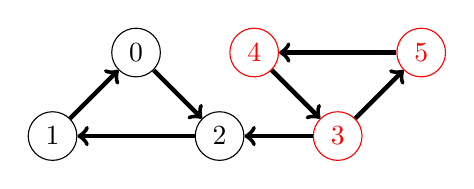
\begin{tikzpicture}[main/.style = {draw, circle}, node distance={15mm},   blacknode/.style={shape=circle, draw=black, line width=2},
                              bluenode/.style={shape=circle, draw=blue, line width=2},
                              greennode/.style={shape=circle, draw=green, line width=2},
                              rednode/.style={shape=circle, draw=red, line width=2}] 
        \node[main] (0) {$0$};
        \node[main] (1) [below left of=0] {$1$};
        \node[main] (2) [below right of=0] {$2$};
        \node[main, red] (3) [right of=2] {$3$};
        \node[main, red] (4) [above left of=3] {$4$};
        \node[main, red] (5) [above right of=3] {$5$};
        \draw[->, ultra thick] (1) -- (0);
        \draw[->, ultra thick] (2) -- (1);
        \draw[->, ultra thick] (0) -- (2);
        \draw[->, ultra thick] (3) -- (2);
        \draw[->, ultra thick] (4) -- (3);
        \draw[->, ultra thick] (5) -- (4);
        \draw[->, ultra thick] (3) -- (5);
    \end{tikzpicture}
    \caption{$G^R$}

    \end{minipage}
    \begin{minipage}{.35\linewidth}
    \centering
    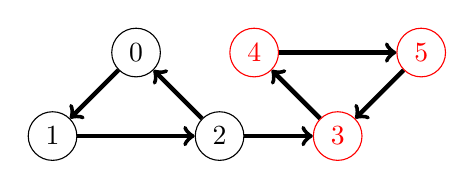
\begin{tikzpicture}[main/.style = {draw, circle}, node distance={15mm},   blacknode/.style={shape=circle, draw=black, line width=2},
                              bluenode/.style={shape=circle, draw=blue, line width=2},
                              greennode/.style={shape=circle, draw=green, line width=2},
                              rednode/.style={shape=circle, draw=red, line width=2}] 
        \node[main] (0) {$0$};
        \node[main] (1) [below left of=0] {$1$};
        \node[main] (2) [below right of=0] {$2$};
        \node[main, red] (3) [right of=2] {$3$};
        \node[main, red] (4) [above left of=3] {$4$};
        \node[main, red] (5) [above right of=3] {$5$};
        \draw[->, ultra thick] (0) -- (1);
        \draw[->, ultra thick] (1) -- (2);
        \draw[->, ultra thick] (2) -- (0);
        \draw[->, ultra thick] (2) -- (3);
        \draw[->, ultra thick] (3) -- (4);
        \draw[->, ultra thick] (4) -- (5);
        \draw[->, ultra thick] (5) -- (3);
    \end{tikzpicture}
    \caption{$G$}
    \end{minipage}

    Running DFS on $G^R$ we can see the highest postorder number will be one of vertices $3, 4, 5$. Let's assume (without loss of generality) tht it is vertex $3$. Running DFS from $3$ will encounter $3, 4, 5$, one SCC. Then running DFS on the rest of the graph, we will get $0, 1, 2$. Note that we could essentially ignore the first SCC once we've found it, since any DFS that reaches it will immediately backtrack. This means we can essentially ignore the $(2, 3)$ edge, such that the second SCC is an 'effective sink' when we run DFS on it.
\end{quickcheck}

\section{Summary}
\begin{summary}
    \begin{itemize}
        \item Graphs
        \begin{itemize}
            \item Tuple of vertices and edges, $G = (V(G), E(G))$.
            \item Can have weights attached to edges using function $f: E(G) \mapsto \mathbb{R}$.
            \item Can be represented by adjacency matrix ($\Omega(n^2)$ space, $O(1)$ edge check) or adjacency list ($O(n + m)$ space, $O(n)$ edge check)
            \item Can be directed/undirected, cyclic/acylic, connected, complete, tree, DAG.
        \end{itemize}
        \item DFS
        \begin{itemize}
            \item Search a graph by repeatedly following edges and backtracking. Runs in $O(n + m)$.
            \item Postvisit and previsit increment shared counter (can be modified, e.g. SCC algorithm)
            \item Four types of edges: tree, forward, back and cross edges.
            \item DFS properties: if $(u, v)$ is a back edge, $postorder(u) < postorder(v)$ and $G$ has a cycle $\iff$ DFS yields a back edge.
            \item DFS can be used to find a topogical sort on a DAG by ordering in decreasing postorder number.
        \end{itemize}
        \item SCCs
        \begin{itemize}
            \item SCCs are maximal vertex sets such that every vertex in the set has a path to every other.
            \item Graph $G'$ with SCCs of $G$ as vertices forms a DAG.
            \item Can find SCCs by running DFS on $G^R$, then running DFS on $G$ and processing vertices in decreasing postorder number from first DFS.
        \end{itemize}
    \end{itemize}
\end{summary}

\newpage
\section{Practice problems}
\subsection{Leetcode practice problems}

\begin{problem}{Programming practice problem 1}
    144. Binary Tree Preorder Traversal (Easy difficulty)
\end{problem}

Python solution using DFS below. Note how for a binary tree we don't need a visited set, we are guaranteed acyclic and connected so a visited set is redundant.

\begin{minted}{python}
def preorderTraversal(self, root: Optional[TreeNode]) -> List[int]:
    lst = []
    def dfs(node: Optional[TreeNode]):
        if not(node):
            return
        lst.append(node.val)
        dfs (node.left)
        dfs (node.right)
    dfs(root)
    return lst
\end{minted}

There are even more condensed (and slightly speedier) solutions, here's one:

\begin{minted}{python}
def preorderTraversal(self, root: Optional[TreeNode]) -> List[int]:
    if not root:
        return []
    return [root.val] + self.preorderTraversal(root.left) + self.preorderTraversal(root.right)
\end{minted}

\begin{problem}{Programming practice problem 2}
    145. Binary Tree Postorder Traversal (Easy difficulty)
\end{problem}

This is a simple modification from the previous part using the first set of code

\begin{minted}{python}
def postorderTraversal(self, root: Optional[TreeNode]) -> List[int]:
    lst = []
    def dfs(node: Optional[ListNode]):
        if not(node):
            return
        dfs(node.left)
        dfs(node.right)
        lst.append(node.val)
    dfs(root)
    return lst
\end{minted}

How can you modify the condensed solution to handle postorder traversal? (\textit{hint: it's just as simple as the modification for the longer solution})

\newpage

\begin{problem}{Programming practice problem 3}
    100. Same Tree (Easy difficulty)
\end{problem}

Python solution:

\begin{minted}{python}
def isSameTree(self, p: Optional[TreeNode], q: Optional[TreeNode]) -> bool:
    if not(p) and not(q):
        return True
    if not(p) or not(q):
        return False
    return p.val == q.val and self.isSameTree(p.left, q.left) and self.isSameTree(p.right, q.right)
\end{minted}

\begin{problem}{Programming practice problem 4}
    695. Max Area of Island (Medium difficulty)
\end{problem}

Python solution using DFS:

\begin{minted}{python}
def maxAreaOfIsland(self, grid: List[List[int]]) -> int:
    self.height = len(grid)
    self.width = len(grid[0])
    max_area = 0

    def dfs(grid: List[List[int]], x: int, y: int):
        if (y < 0 or y >= self.height) or (x < 0 or x >= self.width):
            return 0
        if (grid[y][x] == 0):
            return 0
        # Save space on visited set by rather setting visited locations to 0!
        grid[y][x] = 0
        return 1 + dfs(grid, x + 1, y)\
                 + dfs(grid, x - 1, y)\
                 + dfs(grid, x, y + 1)\
                 + dfs(grid, x, y - 1)

    for y in range(self.height):
        for x in range(self.width):
            if(grid[y][x] == 1):
                max_area = max(dfs(grid, x, y), max_area)
    return max_area
\end{minted}

\newpage

\begin{problem}{Programming practice problem 5}
    302. Smallest Rectangle Enclosing Black Pixels (Hard difficulty)
\end{problem}

Python solution using DFS (\textit{note: I disagree with the presentation of the problem, to me x and y should be flipped but the example makes it clear that x actually relates to height not width}):

\begin{minted}{python}
def minArea(self, image: List[List[str]], x: int, y: int) -> int:
    # Initially given a black pixel
    maxY = minY = y
    maxX = minX = x
    height = len(image)
    width = len(image[0])

    def updateStore(x, y):
        nonlocal maxX, maxY, minX, minY
        maxX = max(x, maxX)
        maxY = max(y, maxY)
        minX = min(x, minX)
        minY = min(y, minY)
    
    def dfs(x: int, y: int):
        if image[x][y] != "1":
            return
        # Rather than visited set, replace all visited pixels! Save some space :)
        image[x][y] = "0"
        updateStore(x, y)
        dfs(min(x + 1, height - 1), y)
        dfs(max(x - 1, 0), y)
        dfs(x, min(width - 1, y + 1))
        dfs(x, max(0, y - 1))
    dfs(x, y)
    # Beware sneaky off-by-1 error
    return (maxX - minX + 1) * (maxY - minY + 1)
\end{minted}

Note that there is a more efficient way to tackle this problem that we will cover later in the course!

\end{document}
